%%%%%%%%%%%%%%%%%%%%%%%%%%%%%%%%%%%%%%%%%%%%%%%%%%%%%%%%%%%%%%%%%%%%%%
% How to use writeLaTeX: 
%
% You edit the source code here on the left, and the preview on the
% right shows you the result within a few seconds.
%
% Bookmark this page and share the URL with your co-authors. They can
% edit at the same time!
%
% You can upload figures, bibliographies, custom classes and
% styles using the files menu.
%
%%%%%%%%%%%%%%%%%%%%%%%%%%%%%%%%%%%%%%%%%%%%%%%%%%%%%%%%%%%%%%%%%%%%%%

\documentclass[12pt]{article}

\usepackage{sbc-template}
\usepackage{graphicx,url}
\usepackage{float}
\usepackage{array}
\usepackage{tabularx}
\usepackage{makecell}

\usepackage{tcolorbox}
\usepackage{minted}

\usepackage[utf8]{inputenc}  

\tcbset{
  codeSnippetStyle/.style={
    colback=gray!10, % cor de fundo mais clara
    colframe=gray!30!, % cor da borda
    title=#1, % título da caixa
    coltitle=black, % cor do título
    boxrule=0.2mm, % espessura da borda
    arc=3mm, % arredondamento dos cantos
    width=\textwidth, % largura da caixa
    boxsep=7pt
  }
}

\newcolumntype{Y}{>{\centering\arraybackslash}X}

\sloppy

%\title{INVESTIGAÇÃO DA ADESÃO DE BOAS PRÁTICAS DE DESENVOLVIMENTO EM PROJETOS OPEN SOURCE FLUTTER: UMA ANÁLISE DE CÓDIGO E MANUTENIBILIDADE}

\title{Análise da Aderência às Boas Práticas de Desenvolvimento em Projetos Open Source Flutter: Primeiros Insights}
\author{Anonymous\inst{1}}

\address{Anonymous \email{\{anonymous\}@anonymous}}

\begin{document} 

\maketitle

\begin{abstract}
This research investigates adherence to best development practices in open-source Flutter projects, focusing on code quality and maintainability. We analyzed 45 projects using SonarQube to identify Best Practice Violations (BPVs). A total of 10,120 BPVs were found, distributed across three severities: 5,149 Minor, 4,273 Major, and 698 Critical. We calculated the Pearson correlation coefficient to confirm the relationship between BPVs and non-commenting lines of code (NCLOC) and between BPVs and cyclomatic complexity. We observed a strong correlation (0.8978) between BPVs and NCLOC, and a moderate correlation (0.4509) between BPVs and complexity. These findings highlight areas for Flutter developers to improve code quality.
\end{abstract}
     
\begin{resumo} 
Esta pesquisa investiga a adesão às melhores práticas de desenvolvimento em projetos open-source Flutter, focando na qualidade e manutenibilidade do código. Analisamos 45 projetos utilizando SonarQube para identificar Violações de Boas Práticas (VBPs). Foram encontradas 10.120 VBPs, distribuídas em três severidades: 5.149 Leves, 4.273 Graves e 698 Críticas. Calculamos o coeficiente de correlação de Pearson para confirmar a relação entre VBPs e linhas de código (LCNC) e entre VBPs e complexidade ciclomática. Observamos uma correlação forte (0.8978) entre VBPs e LCNC, e uma correlação moderada (0.4509) entre VBPs e complexidade. Esses achados destacam áreas para os desenvolvedores Flutter melhorarem a qualidade do código.
\end{resumo}

\section{Introdução}
A evolução tecnológica acelerada tem modificado substancialmente nossa interação com o mundo digital, com os dispositivos móveis emergindo como agentes principais dessa transformação. No Brasil, a média de 1,2 smartphones por habitante causa uma demanda crescente por serviços digitais e aplicativos móveis. Em 2022, por exemplo, os investimentos em tecnologia da informação (TI) corresponderam a 9\% do faturamento das empresas, refletindo também em um aumento significativo no desenvolvimento de aplicativos móveis \cite{FGVcia2023}.

Lançado pelo Google em 2017, o Flutter é um \textit{framework} de código aberto que se tornou popular por permitir que desenvolvedores criem aplicativos que funcionam em múltiplos sistemas operacionais, como Android e iOS, com mínimas alterações no código-fonte, tornando-se uma escolha popular para desenvolvimento multiplataforma \cite{flutter}. Utilizando a linguagem de programação Dart, também desenvolvida pelo Google, o Flutter facilita a escrita de código de alta qualidade e a manutenção a longo prazo. Além disso, se destaca pelo motor gráfico próprio, que oferece consistência e desempenho em diferentes plataformas, e pelo rico ecossistema de pacotes e plugins disponível no Pub, o gerenciador de pacotes do Dart.

Para garantir que os aplicativos desenvolvidos com Flutter mantenham sua robustez e sejam facilmente mantidos ao longo do tempo, é essencial adotar as melhores práticas de desenvolvimento. No contexto do Flutter, isso inclui seguir recomendações da equipe principal do Dart, como legibilidade, consistência, concisão e eficiência do código \cite{dartBestPractices}. Princípios de código limpo, como clareza, simplicidade e eficiência, além de técnicas de refatoração contínua \cite{fowler1999refactoring}, são fundamentais para assegurar a qualidade técnica do software e facilitar sua manutenção contínua.

Neste contexto, as Violações de Boas Práticas (VBPs) são definidas como desvios das diretrizes estabelecidas pela equipe principal do Dart para garantir a escrita de código claro, eficiente e de fácil manutenção. Essas diretrizes estão descritas no guia "Effective Dart", que inclui recomendações sobre estilo, documentação e práticas específicas para desenvolvimento em Dart e Flutter \cite{dartBestPractices}.

Este estudo investiga a adesão às melhores práticas de programação recomendadas pelo time principal do Dart em projetos open source desenvolvidos com Flutter, visando responder as seguintes questões de pesquisa:
\begin{enumerate}
\item Qual a prevalência de violações das melhores práticas recomendadas?
\item Com que frequência essas práticas são violadas?
\item Quais tipos de práticas são mais frequentemente violadas?
\end{enumerate}

\section{Metodologia}

A metodologia adotada foi estruturada em quatro etapas principais: seleção de projetos, configuração das ferramentas de análise, coleta de dados e avaliação dos resultados. Além das VBPs, também analisamos a complexidade do código dos projetos, medida por métricas como a complexidade ciclomática e número de linhas de código não comentadas (LCNC) \cite{mccabe1976complexity}, para avaliar a qualidade dos projetos Flutter.

\subsection{Seleção de Projetos}
A seleção apropriada dos projetos é crucial para garantir a relevância da pesquisa. Inicialmente, foram considerados os projetos open source Flutter recomendados pela comunidade e disponíveis no repositório \textit{Open-Source Flutter Apps}\footnote{Tortuvshin Bayarsaikhan. Open-Source Flutter Apps. 2023. Disponível em: \url{https://github.com/tortuvshin/open-source-flutter-apps}. Acessado em: 08 de julho de 2024}, que contava com 152 projetos em 15 de maio de 2024. Aplicamos critérios específicos para filtrar esses projetos, resultando em uma amostra final de 50 projetos relevantes para análise:
\begin{enumerate}
    \item No mínimo 30 commits, garantindo projetos com um histórico consistente de atividade.
    \item Último commit feito nos últimos 3 anos, assegurando atividade recente.
    \item Mínimo de 30 estrelas no GitHub, indicando relevância na comunidade.
\end{enumerate}


\subsection{Procedimento e Análise dos Resultados}
Utilizamos o SonarQube, uma plataforma reconhecida por sua capacidade de análise de código, para identificar VBPs. O SonarQube foi instalado em um container Docker para garantir um ambiente de análise controlado e consistente. Também configuramos o SonarScanner para coletar dados detalhados dos projetos.

A análise foi realizada utilizando o SonarScanner, configurado com um arquivo \texttt{sonar-project.properties} específico para cada projeto. Foram coletadas métricas como número de VBPs, severidade e complexidade ciclomática. Os seguintes passos foram seguidos para realizar a análise:
\begin{enumerate}
    \item Configuração do ambiente Docker e instalação do SonarQube.
    \item Download e instalação do plugin para análise de Dart e Flutter.
    \item Configuração e execução do SonarScanner nos projetos selecionados.
\end{enumerate}

Durante a fase de análise, 5 projetos foram excluídos devido a problemas técnicos. Entre os problemas encontrados estavam incompatibilidades de versões de dependências, incompatibilidades de bibliotecas e uso de bibliotecas descontinuadas.

Os dados foram coletados através da API do SonarQube e armazenados em formato JSON. Utilizamos scripts em Python para automatizar a coleta, tratamento e análise dos dados, garantindo consistência e precisão nos resultados. 

Os resultados foram analisados para identificar a prevalência e severidade das VBPs. Calculamos o coeficiente de correlação de Pearson para avaliar a relação entre VBPs e Linhas de Código Não Comentadas (LCNC) e entre VBPs e complexidade ciclomática. Os dados foram visualizados por meio de gráficos e tabelas para facilitar a interpretação.

\section{Resultados}

A análise dos 45 projetos open source desenvolvidos com Flutter, utilizando o SonarQube, revelou 10.120 VBPs. Estas foram distribuídas em três níveis de severidade: 5.149 menores, 4.273 maiores e 698 críticas, avaliando a adesão às melhores práticas de desenvolvimento.

\subsection{Correlação entre VBPs, Linhas de Código Não Comentadas (LCNC) e Complexidade Ciclomática}
Calculamos o coeficiente de correlação de Pearson para avaliar a relação entre VBPs e o número de LCNC, bem como entre VBPs e complexidade ciclomática. Na Figura~\ref{fig:vbps_vs_lcnc_and_vbps_vs_complexity}, observamos uma correlação forte (\textit{r} = 0.8978) entre VBPs e LCNC, indicando que mais linhas de código estão associadas a mais VBPs. Adicionalmente, a Figura~\ref{fig:vbps_vs_lcnc_and_vbps_vs_complexity} mostra uma correlação moderada (\textit{r} = 0.4509) entre VBPs e complexidade ciclomática, sugerindo que projetos com maior complexidade ciclomática tendem a ter mais VBPs.

\begin{figure}[H]
\centering
\includegraphics[width=0.45\textwidth]{images/correlação_entre_vbps_e_lcnc.png}
\includegraphics[width=0.45\textwidth]{images/correlação_entre_vbps_e_complexidade_ciclomática.png}
\caption{Correlação entre VBPs e LCNC (esquerda) e entre VBPs e Complexidade Ciclomática (direita)}
\label{fig:vbps_vs_lcnc_and_vbps_vs_complexity}
\end{figure}

\subsection{Regras Mais Violadas}
A Figura~\ref{fig:rule_distribution} mostra a distribuição das cinco regras de boas práticas mais frequentemente violadas nos projetos analisados. A VBP mais frequente foi a EC (\textit{Exhaustive Cases}), com um total de 1544 violações. Esta regra verifica se todas as possibilidades em uma enumeração são cobertas, garantindo que o código seja robusto e não falhe ao encontrar casos inesperados. A alta frequência de violações desta regra indica que os desenvolvedores muitas vezes deixam de tratar todos os casos possíveis em enumerações, o que pode levar a erros em tempo de execução e a um código menos confiável.

\begin{figure}[H]
\centering
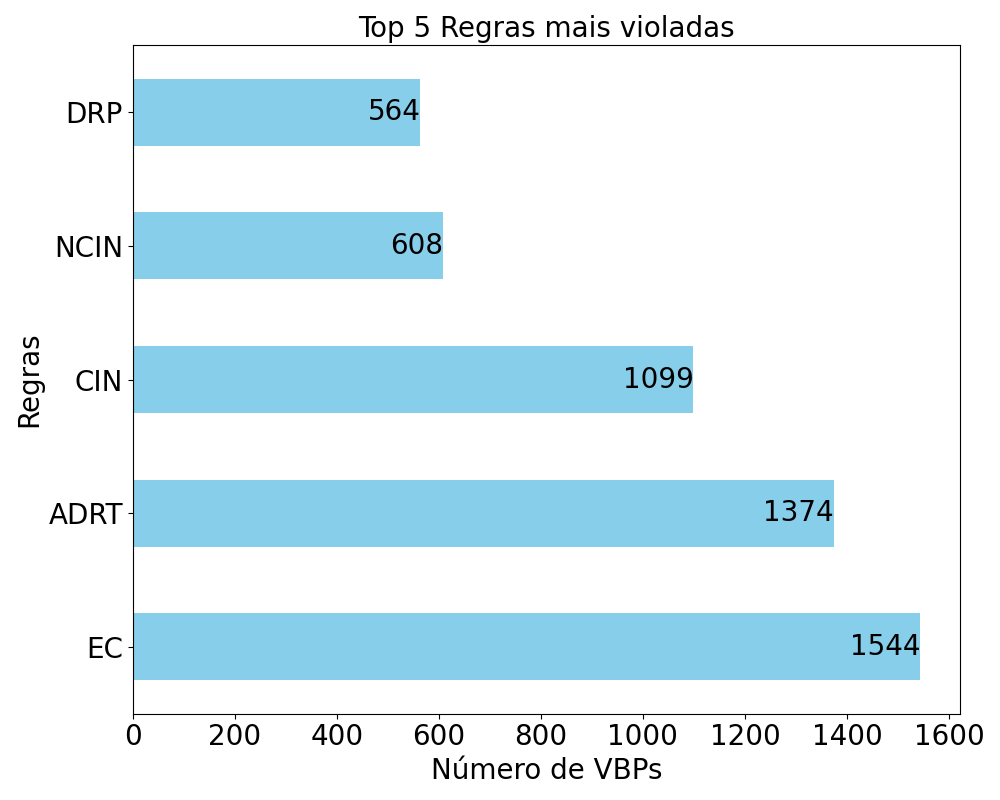
\includegraphics[width=.5\textwidth]{images/rule_distribution.png}
\caption{Distribuição das Regras Mais Violadas}
\label{fig:rule_distribution}
\end{figure}

As siglas usadas no gráfico representam: \textbf{EC}: \textit{Exhaustive Cases}, verifica se todas as possibilidades em uma enumeração são cobertas; \textbf{ADRT}: \textit{Always Declare Return Types}, garante que todas as funções tenham tipos de retorno declarados; \textbf{CIN}: \textit{Constant Identifier Names}, verifica se os nomes das constantes estão em conformidade com as convenções de nomenclatura; \textbf{NCIN}: \textit{Non Constant Identifier Names}, verifica se os nomes dos identificadores não constantes estão em conformidade com as convenções de nomenclatura; \textbf{DRP}: \textit{Depend on Referenced Packages}, garante que as dependências declaradas estejam sendo utilizadas.

\subsection{Exemplo de Violação Crítica: Always Declare Return Types (ADRT)}
Entre as regras mais frequentemente violadas, a prática de declarar explicitamente os tipos de retorno de métodos (\textbf{ADRT}) se destaca por sua importância na manutenção e compreensão do código.

No exemplo abaixo, retirado do repositório \textit{gsy\_github\_app\_flutter} \footnote{CarGuo. gsy\_github\_app\_flutter. Disponível em: \url{https://github.com/CarGuo/gsy\_github_app\_flutter/blob/3b7d9d2618305c8cab036bd11e5e6f9680ab6b00/lib/page/my\_page.dart#L41}. Acessado em: 10 de julho de 2024}, o método \texttt{getUserType}  não possui um tipo de retorno declarado, o que pode levar a problemas de manutenção e compreensão do código:

\begin{tcolorbox}[codeSnippetStyle={gsy\_github\_app\_flutter/lib/page/my\_page.dart}]
\begin{minted}[breaklines, fontsize=\footnotesize]{dart}
getUserType() {
  if (_getStore()?.state.userInfo == null) {
    return null;
  }
  return _getStore()?.state.userInfo?.type;
}
\end{minted}
\end{tcolorbox}

\section{Considerações Finais}
\subsection{Resultados Encontrados}
Esta pesquisa analisou 45 projetos open-source Flutter para identificar Violações de Boas Práticas (VBPs), encontrando mais de 10.000 violações distribuídas entre diferentes severidades.

Esses resultados destacam áreas específicas onde melhorias podem ser feitas para aderir melhor às práticas recomendadas e melhorar a qualidade e manutenibilidade do código em projetos Flutter.

Os resultados desta pesquisa mostram uma forte correlação entre o número de VBPs e as linhas de código não comentadas (LCNC), indicando que projetos maiores tendem a apresentar mais violações. Também foi observada uma correlação moderada entre VBPs e complexidade ciclomática, sugerindo que a complexidade do código influencia a qualidade do software.

As regras mais violadas, como Exhaustive Cases e Always Declare Return Types, indicam áreas onde os desenvolvedores devem concentrar esforços para melhorar a qualidade do código. A utilização de práticas de codificação estruturada é essencial para a manutenibilidade do software, conforme destacado por Hunt e Thomas \cite{hunt1999pragmatic}.

Para reduzir tais violações, uma abordagem eficaz é fomentar o uso de ferramentas de análise estática e verificação de código, como SonarQube e Dart Analyzer, durante o desenvolvimento.  Essas ferramentas podem identificar violações de boas práticas em tempo real, permitindo correções antes que se tornem significativas. A integração dessas ferramentas no processo de desenvolvimento contínuo pode ajudar a manter a qualidade do código, reduzir a complexidade ciclomática e evitar a duplicação de código \cite{measuringCC2023}.

\subsection{Trabalhos Futuros}
Para futuros trabalhos, espera-se realizar uma análise mais detalhada das causas das violações de boas práticas e uma investigação de processos automatizadas para auxiliar os desenvolvedores a aderirem a essas práticas. Outra possibilidade é expandir o conjunto de dados para incluir mais projetos e explorar a eficácia de diferentes ferramentas e metodologias de análise de código.

\bibliographystyle{sbc}
\bibliography{sbc-template}

\end{document}
